%!TEX root = main.tex

\section{Dataset and measures of political behavior}
\label{sec:four-measures}

In this section, we first describe the \debate dataset that we collected during the 1st U.S. presidential debate.
Next, we introduce three measures for analyzing the political behavior of users who were active on Twitter during the debate.
In Sec.~\ref{subsec:political-polarization-measures}, we introduce \emph{political polarization} $\mathcal{P}$ and \emph{political engagement} $\mathcal{E}$.
In Sec.~\ref{subsec:bot-detection} we introduce the \emph{botness score} $\zeta$ and we describe how we construct the reference bot and human populations.
%Finally, in Sec.~\ref{subsec:user-influence-measure} we compute the user influence $\varphi$ based on all retweet cascades in \debate.

%\subsection{The \debate dataset}
%\label{subsec:debatenight-construction}

\textbf{The \debate dataset}
contains Twitter discussions that occurred during the 1st 2016 U.S presidential debate between Hillary Clinton and Donald Trump.
Using the Twitter Firehose API\footnote{Via the Uberlink Twitter Analytics Service.}, we collected all the tweets (including retweets) that were authored during the two hour period from 8.45pm to 10.45pm EDT, on 26 September 2016, and which contain at least one of the hashtags: \texttt{\#DebateNight}, \texttt{\#Debates2016}, \texttt{\#election2016}, \texttt{\#HillaryClinton}, \texttt{\#Debates}, \texttt{\#Hillary2016}, \texttt{\#DonaldTrump} and \texttt{\#Trump2016}.
The time range includes the 90 minutes of the presidential debate, as well as 15 minutes before and 15 minutes after the debate.
The resulting dataset contains 6,498,818 tweets, emitted by 1,451,388 twitter users.
For each user, the Twitter API provides aggregate information such as the number of followers, the total number (over the lifetime of the user) of emitted tweets, authored retweets, and favorites.
For individual tweets, the API provides the timestamp and, if it is a retweet, the original tweet that started the retweet cascade.
The \debate dataset contains 200,191 retweet diffusions of size 3 and larger.
%Using this information, we \rev{used the approach described in Section~\ref{sec:user-influence} to reconstruct} 200,191 complete retweet cascades\footnote{We make sure that no retweets are missing from cascades by checking the \texttt{retweets\_count} field provided by Twitter API.} of size at least 3.
%As the \#DebateNight hashtag accounts for over half of the tweets, we refer to our data as the "\#DebateNight dataset".

\subsection{Political polarization $\mathcal{P}$ and engagement $\mathcal{E}$}
\label{subsec:political-polarization-measures}

%!TEX root = main.tex

%% MAR: the wordclouds were obtained using "https://wordart.com/create"
\begin{figure}[tbp]
	\centering
	\newcommand\mywidth{0.45}
	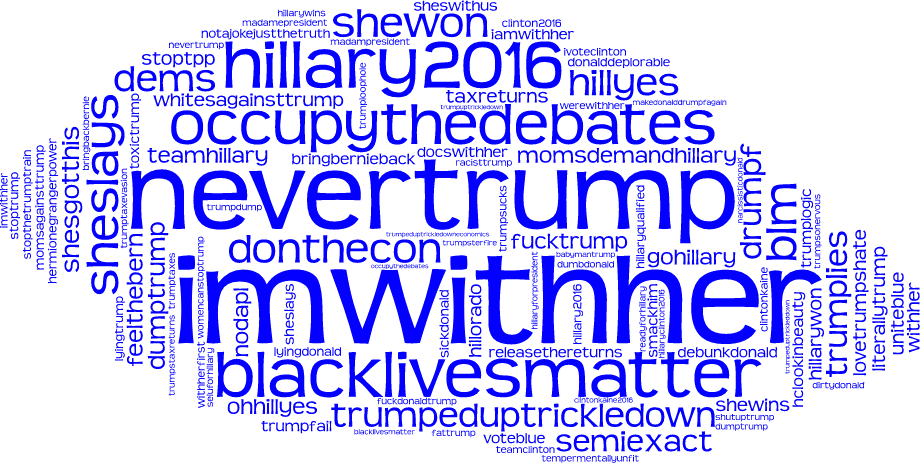
\includegraphics[width=\mywidth\textwidth]{democrat-2} %% also good democrat-4
	\vspace{0.1cm}\\
	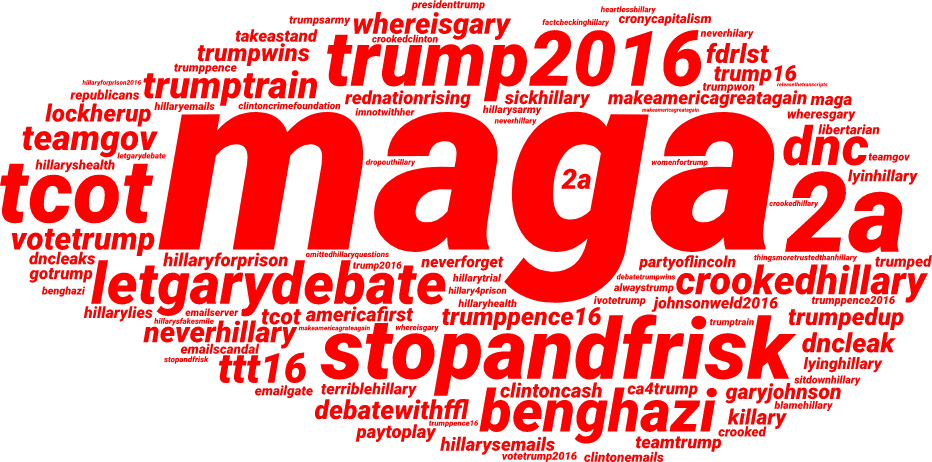
\includegraphics[width=\mywidth\textwidth]{republican-1}
	\caption{
		Wordclouds of partisan hashtags in \debate: Democrat \textbf{(top)} and Republican \textbf{(bottom)}.
		Hashtags sizes are scaled by their frequency.
	}
	\label{fig:wordclouds}
%	\captionmoveup
\end{figure}

%\TODO{@TG}{This paragraph does not make it clear that we ONLY chose ``clearly partisan'' hashtags, and not generally Democrat- or Republican-leaning hashtags.
%This should address inevitable questions about why only 1k tweets have both, and also RJA's remark in Sec 6 about why so little users in the middle of Fig. 4a.
%See text in purple here below.}

\textbf{Protocol.}
Content analysis~\cite{kimkuljis2010} was used to code the 1000 most frequently occurring hashtags according to their political polarity. More specifically, we used 
Directed Content Analysis~\cite{hsieh-shannon-2005} to contextually analyse hashtags and code them according to their political polarity (or not, denoted as `neutral' and subsequently excluded from analysis). 
This approach has been used in previous work to study hashtags on Twitter in a manner that is valid, reliable and replicable~\cite{small-2011}. 
There were two previous studies of Twitter activity during the 2016 U.S. presidential election that informed the development of our coding schema. 
Firstly, \citet{FM7090} devised a binary classification scheme that attributed political partisanship to a small set of key hashtags as either `Trump-supporting' (\#donaldtrump, \#trump2016, \#neverhillary, \#trumppence16, \#trump) or `Clinton-supporting' (\#hillaryclinton, \#imwithher, \#nevertrump, \#hillary). 
Secondly, in studying Twitter activity during the 1st U.S. presidential debate, \citet{Kollanyi.2016.presidentialdebate} developed a coding schema that categorized tweets into seven categories based on the hashtags that occurred within the tweet. 
However, the authors found that three `exclusive' categories (`Pro-Trump', `Pro-Clinton', and `Neutral') accounted for the majority (88.5\%) of observations. 

Given the findings of previous research, we developed a code book with three categories: `Pro-Trump', `Pro-Clinton', and `Neutral'. 
To ensure that hashtags were analyzed within context, our content analysis methodology focussed on three units of analysis (following the approach developed by~\citet{small-2011}). 
The first is hashtags, comprised of a set of the 1000 most frequently occurring hashtags over all tweets in our dataset. 
The second unit of analysis was individual tweets that contained these hashtags. 
In order to gain a more nuanced and `situated' interpretation of hashtag usage, for each hashtag we referred to a small random sample of tweets in our dataset that contained each given hashtag. 
In some instances the polarity (or neutrality) was clear and/or already determined from previous studies, which helped to speed up the analysis of tweets. 
The third unit of analysis was user profiles, which we referred to in situations where the polarity or neutrality of a given hashtag was unclear from the context of tweet analysis. 
For example, \#partyoflincoln was used by both Republican and Democrat Twitter users, but an analysis of both tweets and user profiles indicated that this hashtag was \textit{predominantly} used by Pro-Trump supporters to positively align the Republican Party with the renowned historical figure of President Abraham Lincoln, who was a Republican. 
The content analysis resulted in a subset of 93 pro-Democrat and 86 pro-Republican hashtags (see the wordcloud visualization in Fig.~\ref{fig:wordclouds}), whilst the remaining `neutral' hashtags were subsequently excluded from further analysis.
The resulting partisan hashtag list contains hashtags indicating either strong support for a candidate (e.g., \texttt{\#imwithher} for Clinton and \texttt{\#trump2016} for Trump), or opposition and/or antagonism (e.g., \texttt{\#nevertrump} and \texttt{\#crookedhillary}).
The complete list of partisan hashtags is publicly available in the Github repository.

%% MAR: this is the old shortened version of the protocol (used in submission)
%We extracted the 1000 most frequent hashtags in our dataset. 
%Using a content analysis approach~\cite{kimkuljis2010}, we coded each hashtag into two categories: Democrat and Republican. 
%Hashtags that did not have a clear political polarity were not labeled and thus excluded from analysis. 
%Our coding methodology is similar to previous work~\cite{Kollanyi.2016.presidentialdebate,FM7090},
%%This follows a similar coding methodology to related studies 
%%although rather than starting with a preconceived set of partisan hashtags we derived these from the data. 
%with the difference that we extract candidate hashtags from the data instead of using a predefined set of partisan hashtags.
%Fig.~\ref{fig:wordclouds} presents the wordclouds of the most frequent partisan hashtags, for Democrats (top) and Republicans (bottom).
%We chose hashtags indicating either strong support for a candidate (e.g., \texttt{\#imwithher} for Clinton and \texttt{\#trump2016} for Trump), or opposition and/or antagonism (e.g., \texttt{\#nevertrump} and \texttt{\#crookedhillary}). 
%\rev{Hashtags were coded in the context of the political discussion.
%More details on the coding protocol can be found in the online supplement~\cite[annex~F]{supplemental}.}
%This results in 93 Democrat and 86 Republican hashtags.
%\rev{The list of partisan hashtags is publicly available in the Github repository.}

\textbf{Two measures of political behavior.}
We identify 65,031 tweets in \debate that contain at least one partisan hashtag (i.e., one of hashtags in the reference set of partisan hashtags constructed earlier).
1,917 tweets contain partisan hashtags with both polarities: these are mostly negative tweets towards both candidates (e.g., ``Let's Get READY TO RUMBLE AND TELL LIES. \#nevertrump \#neverhillary \#Obama'') or hashtag spam.
We count the number of occurrences of partisan hashtags for each user, and we detect a set of 46,906 politically engaged users that have used at least one partisan hashtag.
Each politically engaged user $u_i$ has two counts: $dem_i$ the number of Democrat hashtags that $u_i$ used, and $rep_i$ the number of Republican hashtags.
We measure the \emph{political polarization} as the normalized difference between the number of Republican and Democrat hashtags used:
\begin{equation}
	\mathcal{P}(u_i) = \frac{rep_i - dem_i}{rep_i + dem_i}.
\end{equation}
$\mathcal{P}(u_i)$ takes values between $-1$ (if $u_i$ emitted only Democrat partisan hashtags) and $1$ ($u_i$ emitted only Republican hashtags).
We threshold the political polarization to construct a population of Democrat users with $\mathcal{P}(u) \leq -0.4$ and Republican users with $\mathcal{P}(u) \geq 0.4$.
In the set of politically engaged users, there are 21,711 Democrat users, 22,644 Republican users and 2,551 users with no polarization ($\mathcal{P}(u) \in (-0.4, 0.4)$).
%
We measure the \emph{political engagement} of users using the total volume of partisan hashtags included in their tweets $\mathcal{E}(u_i) = rep_i + dem_i$.

\subsection{Botness score $\zeta$ and bot detection}
\label{subsec:bot-detection}

%% MAR: cutting down on the motivation, should be in intro, not here.
%A key problem is how to classify user accounts who participated in \#DebateNight into those who are human versus those who are bots and/or `highly automated' \cite{Kollanyi.2016.presidentialdebate}. The large of number of users in our dataset (over 1.5 million) meant that manual human classification was not possible within a reasonable time-frame and resources\footnote{For instance, if each user took 30 seconds to manually annotate, it would take over 1.5 years for a researcher working 24 hours a day.}. Therefore, we used a state-of-the-art bot detection system known as `BotOrNot', discussed previously in Sec.~\ref{previousworkbots}.

\textbf{Detecting automated bots.}
%Using the BotOrNot API, we classified each of the 1,451,388 users in our dataset to extract their bot scores. 
We use the BotOrNot~\cite{davisetal.16} API to measure the likelihood of a user being a bot for each of the 1,451,388 users in the \debate dataset.
Given a user $u$, the API returns the botness score $\zeta(u) \in [0, 1]$ (with 0 being likely human, and 1 likely non-human).
%Next, we determined a threshold value to decide whether a user is a bot or not. 
%The BotOrNot authors indicate that this is a non-trivial problem due to the varying levels of sophistication of bots and the fact that bots are continuously changing and being modified to thwart detection. 
%As a starting point, we chose a threshold value of 0.5, which the authors indicate provided an overall classification accuracy of 86\% through their cross-validation process (Varol et al., 2017: 283), and is also a threshold used in previous studies \cite{FM7090,Woolley.2017}. 
%In this way, if a user scored above 0.5 then they were classified as a bot. 
Previous work~\cite{varol.17,FM7090,Woolley.2017} use a botness threshold of $0.5$ to detect socialbots.
However, we manually checked a random sample of 100 users with $\zeta(u) > 0.5$ and we found several human accounts being classified as bots.
A threshold of 0.6 decreases mis-classification by $3\%$.
%whilst raising the threshold to 0.6 provided more accurate results. 
%we therefore employ a threshold of $0.6$ to differentiate bot-like accounts.
%We observed that a number of organizational accounts were misclassified as bots. 
It has been previously reported by \citet{varol.17} that organizational accounts have high botness scores.
%This issue relating to misclassification of organizational accounts was reported by \cite[p. 2]{varol.17}. 
This however is not a concern in this work, as we aim to detect 
%However, this was not a concern as we were not only interested in bots but also 
`highly automated' accounts that behave in a non-human way. 
We chose to use a threshold of $0.6$ to construct the \Bot population in light of the more encompassing notion of account \emph{automation}. 
%On the other hand, manual analysis of a small random sample of `human' accounts (with scores $<= 0.6$) showed that setting a threshold of 0.2 allowed us to classify accounts as almost certainly human (operated by a single living individual). 
%We then converted the bot scores over all users into a dichotomous variable, i.e., 0 for human; 1 for bot) and applied it to our network as a node attribute for further analysis.

%!TEX root = main.tex

%% latex table generated in R 3.4.0 by xtable 1.8-2 package
%% Thu Nov 30 17:07:53 2017
%\begin{table}[tb]
%	\renewcommand{\cellalign}{cr}
%	\scriptsize
%%	\fontsize{6.5pt}%{10.0pt}
%%	\selectfont
%	\setlength{\tabcolsep}{5pt}
%	\centering
%	\caption{
%		Tabulating population volumes and percentages of politically polarized users over four populations: \Protected, \Human, \Suspended and \Bot.
%%		Retrieving botness score failed for 4,822 users.
%	}
%	\begin{tabular}{rr|rrr|rr}
%		\toprule
%			& All & Polarized & Dem. & Rep. & Dem. \% & Rep. \% \\ 
%  		\midrule
%			All & 1,451,388 & 44,299 & 21,676 & 22,623 & 48.93\% & 51.07\% \\ 
%  			\Protected & 45,316 & 1,245 & 585 & 660 & 46.99\% & 53.01\% \\ 
%			\makecell{\Human\\($\zeta \leq 0.2$)} & 499,822 & 11,972 & 5,376 & 6,596 & 44.90\% & 55.10\% \\ 
%  			\Suspended & 10,162 & 265 & 111 & 154 & 41.89\% & 58.11\% \\ 
%  			\makecell{\Bot\\($\zeta \geq 0.6$)} & 17,561 & 435 & 185 & 250 & 42.53\% & 57.47\% \\ 
%   		\bottomrule
%	\end{tabular}
%	\label{tab:populations-effectives}
%	\captionmoveup
%\end{table}

% MAR: one idea is to transpose this table, because the scriptsize above is ugly.
%		But extra work is required.
% latex table generated in R 3.4.0 by xtable 1.8-2 package
% Thu Nov 30 17:07:53 2017
\begin{table}[tb]
	\renewcommand{\cellalign}{cr}
	\small
	\setlength{\tabcolsep}{4pt}
	\centering
	\caption{
		Tabulating population volumes and percentages of politically polarized users over four populations: \Protected, \Human, \Suspended and \Bot.
%		Retrieving botness score failed for 4,822 users.
	}
	\begin{tabular}{rrrrrr}
		\toprule
			& All & \texttt{Prot.} & \Human & \texttt{Susp.} & \Bot \\
  		\midrule		
			All & 1,451,388 & 45,316 & 499,822 & 10,162 & 17,561 \\
			Polarized & 44,299 & 1,245 & 11,972 & 265 & 435 \\
			Democrat & 21,676 & 585 & 5,376 & 111 & 185 \\
			Republican & 22,623 & 660 & 6,596 & 154 & 250 \\
		\midrule
			Dem. \% & 48.93\% & 46.99\% & 44.90\% & 41.89\% & 42.53\%\\
			Rep. \% & 51.07\% & 53.01\% & 55.10\% & 58.11\% & 57.47\%\\ 
   		\bottomrule
	\end{tabular}
	\label{tab:populations-effectives}
%	\captionmoveup
\end{table}

\textbf{Four reference populations.}
In addition to the \Bot population, we construct three additional reference populations:
%, based on the ``BotOrNot'' API \cite{varol.17}. \emph{Bot} have a bot score $\ge 0.6$; users in this population have a high likelihood of being automated bots and institutional accounts.
\Human $\zeta(u) \leq 0.2$ contains users with a high likelihood of being regular Twitter users.
\Protected are the users whose profile has the access restricted to their followers and friends (the BotOrNot system cannot return the botness score); we consider these users to be regular Twitter users, since we assume that no organization or broadcasting bot would restrict access to their profile.
\emph{Suspended} are those users which have been suspended by Twitter between the date of the tweet collection (26 September 2016) and the date of retrieving the botness score (July 2017);
this population has a high likelihood of containing bots.
%, given the crackdown on bots performed by Twitter~\verify{\textbf{\hl{[ref?]}}}.
% TIM COMMENT: If we want a Twitter reference for this, we could use: https://blog.twitter.com/official/en_us/topics/company/2017/Our-Approach-Bots-Misinformation.html
%\verify{RJA comment: What \% were bots, humans, and neither?}
Table~\ref{tab:populations-effectives} tabulates the size of each population, split over  political polarization.
